\section{Deployment}

\subsection{Versioned Product Surface}

The public artifact at \url{https://github.com/CSTCloudOps/TShape-Zero} packages the strict checkpoint, shared scorer, CLI, and web interface as one versioned product. The checkpoint metadata records Pattern Bank version and size, seed, preprocessing, stopping rule, fusion weights, and SHA256 digest. A verification ledger maps every reported cell to method status, valid-series count, coverage, and metric implementation. Dataset licenses are respected through acquisition instructions and a checksum manifest rather than silent redistribution.

\begin{figure}[t]
  \centering
  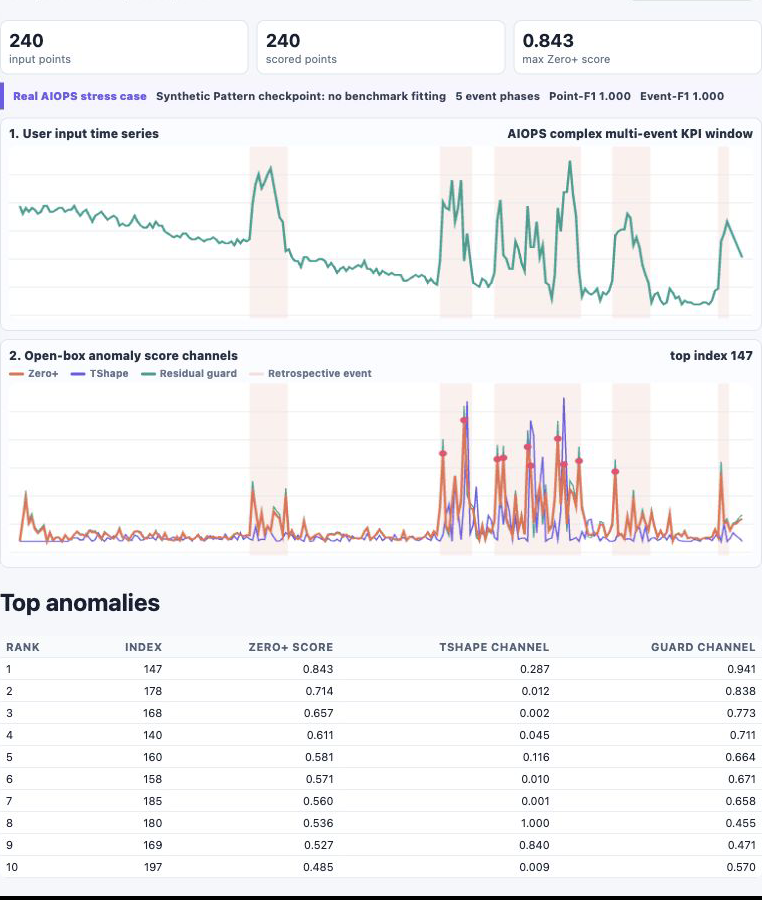
\includegraphics[width=\columnwidth]{figures/fig_product_strict_panel.png}
  \caption{Released web scorer on a complex real 240-point AIOPS incident window. The interface returns the aligned KPI trace, fused/neural/guard scores, and ranked suspicious points from the same scorer used by the CLI.}
  \label{fig:product}
\end{figure}

Fig.~\ref{fig:product} shows the product path on a real AIOPS window with baseline drift and five anomaly phases, including bursts, plateaus, partial recoveries, and renewed excursions. The user pastes or uploads history and may optionally provide a separate unlabeled calibration prefix. The service validates numeric input, applies the documented difference-and-scale contract, runs the frozen 0.138-MiB checkpoint and three guard channels, restores raw-index alignment, and returns two linked plots plus a top-$k$ table. No target label, gradient step, or target-specific checkpoint selection occurs.

For this 240-point case, \method{} obtains retrospective local \pfone{} 1.000 and \efone{} 1.000, and all ten highest-scored points lie inside labeled incident phases. The case is intentionally demanding rather than a single isolated spike. It was selected for interface demonstration only after the model and aggregate evaluation were frozen; its values, labels, channel scores, and selection rule are included so reviewers can reproduce the screenshot and recognize that it is not a held-out statistical result.

The deployment contract exposes failure rather than hiding it. The default response returns continuous scores and component attribution, not an EasyTSAD oracle threshold. Invalid or too-short histories fail with an actionable message. The reviewer workflow verifies metric conformance without data, scores a bundled smoke trace, regenerates the case, and then optionally executes the full 834-series tier. CLI and web requests share one scoring function, so interface drift cannot silently change the paper result. The current release is a batch historical scorer; causal streaming normalization and automated paging policy are explicit future contracts.

\subsection{Executable Deployment Contract}

Table~\ref{tab:deployment-contract} makes the product boundary testable. A request contains a numeric univariate history and may contain a separate unlabeled calibration prefix. The service rejects malformed values and histories shorter than the model context. A successful response has the same raw index space as the upload and contains the fused score, neural score, guard score, ranked indices, and immutable model metadata. The one-point differencing warm-up is restored as a non-alarming pad rather than silently shifting incident locations. This alignment check is important in operations, where an off-by-one alert can associate an anomaly with the wrong deployment or log window.

\begin{table}[t]
\caption{Executable product and reviewer contract.}
\label{tab:deployment-contract}
\centering
\scriptsize
\setlength{\tabcolsep}{3.0pt}
\begin{tabular}{>{\raggedright\arraybackslash}p{0.20\columnwidth}>{\raggedright\arraybackslash}p{0.39\columnwidth}>{\raggedright\arraybackslash}p{0.31\columnwidth}}
\toprule
Contract & Shipped behavior & Verification assertion \\
\midrule
Checkpoint & 145,215 bytes; immutable metadata and digest & Hash and strict-training flags match \\
Input & Numeric history; optional unlabeled calibration prefix & Malformed and short inputs fail \\
Alignment & Warm-up pad restores raw upload indices & Output length equals input length \\
Evidence & Fused, neural, guard, and ranked suspicious points & Fixed fusion recomputes exactly \\
Labels & Never accepted by the scoring path & Case labels are overlay-only \\
Coverage & One checkpoint for all six benchmark families & Ledger contains 834/834 series \\
\bottomrule
\end{tabular}
\end{table}

The open-box response also supports an operational decision rule without pretending to solve alarm policy. When neural and guard channels agree at a top-ranked point, the operator receives two independent forms of evidence. A guard-dominated point indicates a sharp level, spectral, or robust-deviation change that the learned channel may not recognize; this is the intended reliability-floor behavior. A neural-dominated point indicates a shape-continuation violation not fully explained by the residual controls. Repeated disagreement is not hidden by the fused score: it is a signal to inspect preprocessing, provide a representative unlabeled calibration history, or fall back to target training before connecting the detector to paging.

\subsection{Reviewer Workflow and Release Tiers}

The release provides three verification tiers. The no-data tier checks the checkpoint digest, score formula, output alignment, deterministic smoke trace, and exact EasyTSAD adapter on boundary and randomized inputs. The case tier regenerates Fig.~\ref{fig:product} from the bundled 240-point history and verifies the displayed top-$k$ ordering and component scores. The full tier acquires each dataset from its documented source, verifies checksums, executes all 834 series, and rebuilds the 44-by-6 ledger, paired intervals, tables, and figures. Each tier emits a machine-readable report, so a reviewer can distinguish ``the interface runs'' from ``the complete empirical claim was reproduced.''

For an SRE team, the recommended present use is historical triage or shadow deployment. The product immediately ranks suspicious regions and exposes why they were ranked; the team then chooses a top-$k$, source-calibrated, or policy-specific alarm threshold using its own false-alert budget. If storage and cold-start cost are secondary, Table~\ref{tab:all-easytsad} shows that a large forecasting foundation checkpoint may be preferable on some KPIs. If a stable target history and retraining budget exist, target-trained TShape remains valid. The release therefore turns empirical heterogeneity into a concrete choice among compact out-of-the-box triage, a larger foundation checkpoint, and target-specific training.
